\section{Featuring New Mapping Needs in RML: Support for RDF-star Construction}
\label{sec:chp4_rml_star}

As the technologies revolving around knowledge graphs advance, so do the needs and requirements for their construction. Taking for instance the W3C Recommendation R2RML~\parencite{das2012r2rml}, it was only focused on RDF construction from relational databases on its release in 2012. A growing number of extensions were published over the years to widen its possibilities. These proposals only extended its features to describe additional data sources~\parencite{DBLP:conf/webist/MichelDFM15,VanAssche2021LeveragingWebThings}, but also to increase its expressiveness regarding the inclusion of data transformation functions~\parencite{de2020implementation,debruyne2016r2rmlf,junior2016funul,kyzirakos2018geotriples}, the generation of more RDF terms (e.g., collections and containers)~\parencite{DBLP:conf/webist/MichelDFM15,debruyne2017R2RML-collections} and RDF-star graphs~\parencite{delva2021rml-star,sundqvist2022extending}. 

As a consequence of these growing needs, the W3C Knowledge Graph Construction Community Group was launched\cref{foot:kgc}. 
Since its inception, this community has gathered the new requirements for KG construction, published them as Mapping Challenges (see \cref{sec:chp4_mapping_challenges}), and started implementing them in the widely adopted RML mapping language. 
The result of these efforts is materialized in a new revision of RML~\parencite{iglesias2023rml}. 
The language is now published as a modular ontology, integrating: (i) extended possibilities in triple generation (RML-Core)~\parencite{core_ontology}; (ii) enriched description of data sources and output targets (RML-IO)~\parencite{io_ontology}; (iii) generation of RDF collections and containers (RML-CC)~\parencite{cc_ontology}; (iv) accurate description of data transformation functions (RML-FNML)~\parencite{fnml_ontology}; and (v) generation of RDF-star graphs (RML-star)~\parencite{star_ontology}.

Thus, this language is comprised of five different modules. 
For each module, there are more resources associated besides the ontology: its requirements, a specification with the module's details with examples and the restrictions written in SHACL shapes to validate mapping documents. 
All associated resources of this new version of RML are gathered in the ontology portal\footnote{\url{https://w3id.org/rml/portal}}. 
In addition, the semantics of the relationships between the old and this new specification are defined and available online\footnote{\url{https://w3id.org/rml/portal/backwards-compatibility}} to facilitate backwards compatibility.

This section focuses on presenting one of the abovementioned modules, RML-star, that enables the generation of RDF-star graphs.  The essential context about RDF reification is first introduced, followed by the motivation and description of the module and its validation. Finally, the adoption that this module had since its inception is shown, both the implementations and produced graphs. 





%In the late years, the RDF-star~\parencite{hartig2017foundations} approach for reification has gained popularity. Along with its expansions, different semantic web technologies have been updated to include this new syntax\footnote{\url{https://w3c.github.io/rdf-star/implementations}}. This section describes one of these updates related to building RDF-star graphs: RML-star. \ana{esto no liga del todo bien con lo anterior}


%Making statements about statements in RDF has posed a challenge since the inception of RDF.
%The first W3C Recommendation of RDF~\parencite{lassila1999rdf} already included a description of the standard reification approach to tackle this issue.
%Other alternatives were proposed over the years, such as named graphs~\parencite{carroll2005namedgraphs}, N-ary relationships~\parencite{naryw3c2006}, singleton properties~\parencite{nguyen2014don}, RDF$^+$~\parencite{schueler2008querying}, and more recently, \mbox{RDF-star}~\parencite{hartig2017foundations}, which is currently being incorporated in the RDF 1.2 specification~\parencite{hartig2023rdf}. 

%RDF-star does not leverage the characteristics of RDF as the others proposals. Instead it extends the RDF syntax to introduce the notion of \texttt{quoted triples}. This approach is currently under development to become a W3C standard\footnote{\url{https://www.w3.org/groups/wg/rdf-star}}. 
%As a consequence, an increasing number of semantic technologies are supporting this proposal\footnote{\url{https://w3c.github.io/rdf-star/implementations}}, which include triplestores (e.g., GraphDB, AnzoGraph) and programming libraries (e.g. Apache Jena, Oxigraph).

%\textcolor{red}{It is possible to construct reified RDF graphs using mappings with the reification approaches abovementioned, except for RDF-star. As this proposal extends the original RDF syntax, it requires mapping languages to adapt and evolve in order to construct RDF-star graphs. This chapter presents the extension of the RML language to enable the construction of RDF-star graphs, RML-star. We first introduce how reified RDF graphs can be constructed using RML with different reification approaches, and then we present RML-star. This proposal is validated with \mbox{Morph-KGC$^{star}$}, a KG construction engine that implements our proposal.}

%This section describes popular reification approaches and shows how they can be used in RML and RML-star with a running example. 
%Standard reification and singleton properties are considered in Section \ref{sec:chp4_validation}, showing that \mbox{Morph-KGC$^{star}$} does not add any overhead in the time required to generate the \mbox{RDF-star} triples compared to them.



\begin{figure*}[!t]
\centering
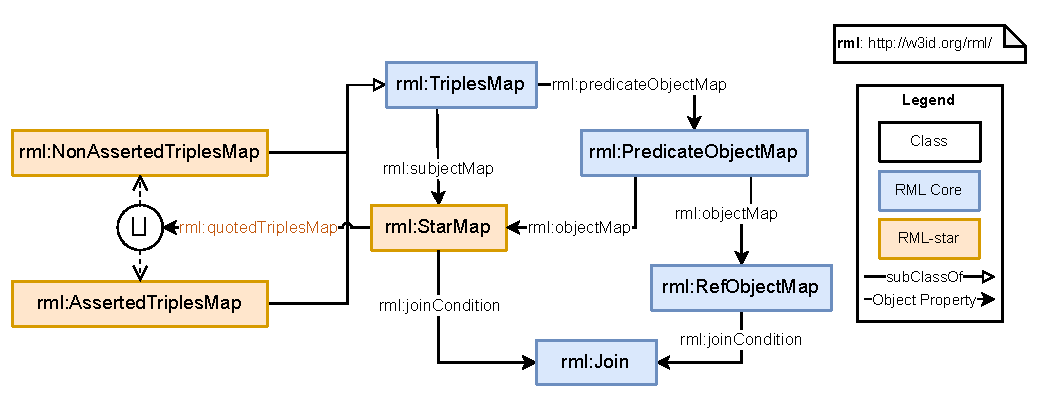
\includegraphics[width=1\linewidth]{figures/chp4-3_rml-star_diagram.pdf}
\caption[RML-star module]{The \mbox{RML-star} module (represented using the Chowlk notation~\parencite{feria2022chowlk}). The RML-star resources are highlighted in orange, while the rest of the represented ontology belongs to the RML-Core module.}
\label{fig:chp4-3_rml-star}
\end{figure*}

\subsection{Reification with RML-star}
\label{sec:chp4_reif_mappings}

%RDF-star has gained adoption over the years since its inception~\parencite{hartig2017foundations}. We propose RML-star as a module of RML to enable the generation of \mbox{RDF-star} graphs (\cref{fig:chp4-3_rml-star}). 


\mbox{RML-star} (\cref{fig:chp4-3_rml-star}) adds a new kind of term map, the \texttt{rml:StarMap}, that allows using triples maps to generate quoted triples. 
Following the \mbox{RDF-star} data model,
a quoted triple may appear only in the subject or object of a triple.
Thus, star maps can only be used in subject and object maps.
Star maps use the property \texttt{rml:quotedTriplesMap} to refer to the triples map that generates the quoted triples. 
The referenced triples map can only be one of the following: (i) \texttt{rml:AssertedTriplesMap} to be asserted in the output graph, or (ii) \texttt{rml:NonAssertedTriplesMap} to not be asserted. A quoted triples map can specify \texttt{rml:class} in the subject map or have multiple predicate-object maps.
Thus, several triples sharing the same subject map and logical source can be quoted by the same star map.







An example of an \mbox{RML-star} mapping rule is shown in \cref{lst:chp4_rml-star}, which generates the \mbox{RDF-star} triples in \cref{lst:chp4_res-rml-star}.
The example uses the data in \cref{lst:chp4_csv_star}, that contains CSV data related to pole vault:
the vaulter (\texttt{PERSON}),
the height of the jump (\texttt{MARK}) and its score (\texttt{SCORE}),
the date when the jump was performed (\texttt{DATE}) and
an identifier of the jump (\texttt{ID}).
%The running example represents that a person jumped some height on a specific date, i.e., it adds the metadata about ``date'' to the statement ``a person jumped some height''.

\noindent\hspace{0.15\linewidth}\begin{minipage}{\linewidth}
\begin{captionedlisting}{lst:chp4_csv_star}{Contents of the logical source \texttt{:marks} in CSV format.}
\centering
\begin{tabular}{c}
\hspace{3em}
{\begin{lstlisting}[basicstyle=\ttfamily\small,label={list:example1},columns=flexible]
ID ,  DATE       ,  MARK ,  PERSON   ,  SCORE
1  ,  2022-03-21 ,  4.80 ,  Angelica ,  1211
2  ,  2022-03-19 ,  4.85 ,  Katerina ,  1224
\end{lstlisting}}
\end{tabular}
\end{captionedlisting}
\end{minipage}

The mapping rules use an asserted triples map (\texttt{<\#jumpTM>}) within the subject map of a triples map (\texttt{<\#dateTM>}). The quoted triples map \texttt{<\#jumpTM>} contains two predicate-object maps that produce triples annotated with \texttt{:date}. The first predicate-object map (\textit{lines 6-9}) produces the triples for the height of the jump, the same as the examples presented previously for the other reification approaches. We extend the RML-star example with a second predicate-object map to also represent the score of the jump within the same quoted triples map (\textit{lines 10-13}). To produce this triple in the other reification approaches an additional triples map for each case would be required.




\noindent\hspace{0.06\linewidth}\begin{minipage}{1\linewidth}
\begin{captionedlisting}{lst:chp4_rml-star}{Example RML-star mapping that transforms data in Listing~\ref{lst:chp4_csv_star}.}
\centering
\begin{tabular}{cc}
\hspace{-2em}{\begin{lstlisting}[basicstyle=\ttfamily\small,label={list:example1},language=rmlstar]
<#jumpTM> 
  a rml:AssertedTriplesMap ;
  rml:logicalSource :marks ;
  rml:subjectMap [ 
    rml:template ":{PERSON}" ] ;
  rml:predicateObjectMap [ 
    rml:predicate :jumps ;
    rml:objectMap [
      rml:reference "MARK" ] ] ;
\end{lstlisting}}
&
\hspace{3em}{\begin{lstlisting}[basicstyle=\ttfamily\small,label={list:example1},firstnumber=14,language=rmlstar]
<#dateTM> 
  a rml:TriplesMap ;
  rml:logicalSource :marks ;
  rml:subjectMap [ 
    rml:quotedTriplesMap <#jumpTM> ] ;
  rml:predicateObjectMap [ 
    rml:predicate :date ;
    rml:objectMap [
      rml:reference "DATE" ] ] .
\end{lstlisting}}\\
\hspace{-2em}{\begin{lstlisting}[basicstyle=\ttfamily\small,label={list:example1},frame=l,rulecolor=\color{red},framerule=0.75pt,firstnumber=10]
  rml:predicateObjectMap [ 
    rml:predicate :score ;
    rml:objectMap [
      rml:reference "SCORE" ] ] .
\end{lstlisting}}

\end{tabular}
\end{captionedlisting}
\end{minipage}


\noindent\hspace{0.1\linewidth}\begin{minipage}{\linewidth}
\begin{captionedlisting}{lst:chp4_res-rml-star}{RDF-star triples generated by the mapping in Listing~\ref{lst:chp4_rml-star}.}
\centering
\begin{tabular}{c}
\hspace{2em}
{\begin{lstlisting}[basicstyle=\ttfamily\small,label={list:example1},columns=flexible]
:Angelica :jumps "4.80" .
<< :Angelica :jumps "4.80" >> :date "2022-03-21" .
:Katerina :jumps "4.85" .
<< :Katerina :jumps "4.85" >> :date "2022-03-19" .
\end{lstlisting}}\\
\hspace{2em}
{\begin{lstlisting}[basicstyle=\ttfamily\small,label={list:example1},columns=flexible,frame=l,rulecolor=\color{red},framerule=0.75pt,firstnumber=5]
:Angelica :score "1211" .
<< :Angelica :score "1211" >> :date "2022-03-21" .
:Katerina :score "1224" .
<< :Katerina :score "1224" >> :date "2022-03-19" .
\end{lstlisting}}

\end{tabular}
\end{captionedlisting}
\end{minipage}


Currently, the \mbox{RML-star} specification~\parencite{iglesias2022rmlstar} provides a complete description of the language, is published as a W3C Draft Community Group Report, and is maintained by the W3C Knowledge Graph Construction Community Group\cref{foot:kgc}. 
This extension belongs to the modules that comprise the new RML specification\footnote{\label{foot:rml-portal}\url{http://w3id.org/rml/portal/}} that is currently under development by the aforementioned Community Group. 
Both the language and the specification are kept up-to-date reflecting the modifications in \mbox{RDF-star}.
For instance, the latest \mbox{RML-star} releases update the term ``embedded'' to ``quoted'',
according to the modifications in \mbox{RDF-star}.
%that occurred after the first release of RML-star~\footnote{\url{https://kg-construct.github.io/rml-star-spec/20210706/}}. 
This update renamed the property \texttt{rml:embeddedTriplesMap} to \texttt{rml:quotedTriplesMap}.
In addition, RML-star is implemented by Morph-KGC$^star$~\parencite{arenas2023morphstar} and the SDM-RDFizer~\footnote{\url{https://github.com/SDM-TIB/SDM-RDFizer-Star}}~\parencite{iglesias2020rdfizer} at the time of writing this document.




\subsection{Validation}
\label{sec:chp4_validation}

This section validates RML-star with (i) the development of the RML-star test-cases, that enables new implementations to check their conformance to RML-star; and (ii) the creation of RML-star mappings for two real-world use cases: software metadata extraction~\parencite{kelley2021framework} (SoMEF) and biomedical research literature~\parencite{SemMedDB} (SemMedDB). 
%We use for both cases \mbox{Morph-KGC$^{star}$}, an implementation of RML-star.




\subsubsection{RML-star Test Cases}
\label{sec:chp4_star_testcases}

Test cases are commonly used %in standardization processes 
to evaluate the conformance of an engine with respect to a language specification (e.g., RML test cases~\parencite{heyvaert2019conformance}). 
A set of \mbox{RDF-star} test cases was proposed
covering the syntax of various of its serializations\footnote{\url{https://w3c.github.io/rdf-star/tests/}}.
We adapted these test cases to create the RML-star test cases and evaluate the conformance of \mbox{Morph-KGC$^{star}$}
with respect to \mbox{RML-star}.

To create a representative set of test cases for \mbox{RML-star}, we selected the N-Triples-star syntax tests\footnote{\url{https://w3c.github.io/rdf-star/tests/nt/syntax}}.  %;and follow a reverse engineering process. 
For each \mbox{RDF-star} test case, we created two associated \mbox{RML-star} test cases that generate the original \mbox{RDF-star} dataset: one test case with a single input data source (i.e., the mapping does not include joins) and another with two input data sources (i.e., the mapping includes joins among triple maps).
For each test case, we manually created the input source(s) in the CSV format and the corresponding \mbox{RML-star} mapping rules to generate the output \mbox{RDF-star} datasets.
Following this approach, we obtained 16 \mbox{RML-star} test cases.
The test cases are openly available\footnote{\url{https://github.com/kg-construct/rml-star/tree/main/test-cases}},
and can be reused by any engine to test its conformance with respect to \mbox{RML-star}.


\subsubsection{Use Cases}
\label{sec:chp4_star_usecases}

We create RML-star mappings for in two real-world use cases. 
The first generates \mbox{RDF-star} graphs from scientific software documentation~\parencite{iglesias2023fair-software-bp}, 
and the second annotates statements extracted from biomedical research publications. 
For both use cases, we use the tool \mbox{Morph-KGC$^{star}$}. 









%In order to ensure that these results in terms of time are representative, we run each mapping three times and calculate the average time.

%In both use cases we report the time on generating the RDF-star datasets. 




%In summary, our test and use cases show that \mbox{Morph-KGC$^{star}$} generates valid RDF triples and does not add an overhead in the generation time of reified triples. However, a more thorough analysis (out of the scope of this paper) is required to describe the behaviour of each mapping approach.

\noindent\textbf{\textit{Scientific Software Metadata Extraction.}}
Scientific software has become a crucial asset to deliver and reproduce the results described in research publications~\parencite{chue_hong_fair_2021}. However, scientific software is often time consuming to understand and reuse due to incomplete and heterogeneous documentation, available only in a human-readable manner.
The Software Metadata Extraction Framework (SoMEF)~\parencite{somef} proposes an approach to automatically extract relevant metadata (description, installation instructions, citation, etc.) from code repositories and their documentation. SoMEF includes different text extraction techniques (e.g., supervised classification, regular expressions, etc.) that yield results with different confidence values.
For example, \cref{lst:JSONsnippet} shows a JSON snippet with the description that SoMEF obtained from a software repository (Widoco) using the GitHub API.
The confidence in this case is high as the extracted description was manually curated by the creators of the code repository.
SoMEF extracts more than 30 different metadata fields about 
software, its source code, its released versions, and their corresponding authors. For transforming the output of SoMEF into RDF-star, we used a total of 35 triples maps to annotate software metadata fields and an additional triples map to annotate source code descriptions. All reified triples follow the same structure (Listings \ref{lst:JSONsnippet} \& \ref{lst:TTLsnippet}), i.e., the standard RDF triple contains the excerpt of the extracted feature, and it is annotated
with the \emph{technique} used and the \emph{confidence} value. 
The complete mapping and all input examples and results are available online\footnote{\url{https://github.com/oeg-upm/rdf-star-generation}}.
 
\noindent\hspace{0.07\linewidth}\begin{minipage}{0.9\linewidth}
\begin{captionedlisting}{lst:JSONsnippet}{JSON snippet showing the description metadata field extracted by SoMEF on a code repository using the GitHub API as extraction technique.}
\centering
\hspace{3em}
{
\begin{lstlisting}[basicstyle=\ttfamily\small,label={list:example1},columns=flexible]
"codeRepository": "https://github.com/oeg-upm/Chowlk",
"description": [ 
 {
  "confidence": 1.0,
  "excerpt": "Tool to transform an ontology diagram into OWL code.",
  "technique": "GitHub API"
 }
]  
\end{lstlisting}
}
\end{captionedlisting}
\end{minipage}

Capturing the technique used and the confidence obtained for each extracted metadata field is key for obtaining an accurate representation of the result. Hence, the \mbox{RDF-star} representation corresponding to the JSON in \cref{lst:JSONsnippet} includes this information, as depicted in \cref{lst:TTLsnippet}.

%\begin{minipage}{0.9\linewidth}
%\begin{captionedlisting}{lst:TTLsnippet}{N-Triples-star snippet showing the results generated for the %description field shown in \cref{lst:JSONsnippet}. Each asserted triple is annotated with its %corresponding confidence and technique.}
%\centering
%\begin{tabular}{c}
%\hspace{1.4em}
%{
%\begin{lstlisting}[numbers=left]
%<< <https://example.org/oeg-upm/Widoco> <https://w3id.org/okn/o/sd#description> 
%    "Wizard for documenting ontologies. WIDOCO is ..." >> 
%        <https://www.w3id.org/okn/o/em#technique> "GitHub API" .
%<< <https://example.org/oeg-upm/Widoco> <https://w3id.org/okn/o/sd#description> 
%    "Wizard for documenting ontologies. WIDOCO is ..." >> 
%        <https://www.w3id.org/okn/o/em#confidence> "1.0" .
%<https://example.org/oeg-upm/Widoco> <https://w3id.org/okn/o/sd#description> 
%    "Wizard for documenting ontologies. WIDOCO is ..." .
%\end{lstlisting}
%}
%\end{tabular}
%\end{captionedlisting}
%\end{minipage}        


\begin{captionedlisting}{lst:TTLsnippet}{RDF-star triples snippet showing the results generated for the description field in \cref{lst:JSONsnippet}. Each asserted triple is annotated with its corresponding confidence and technique.}
\centering
{
\begin{lstlisting}[basicstyle=\ttfamily\small,label={list:example1},columns=flexible]
<oeg-upm/Chowlk> :description "Tool to transform an ontology diagram into OWL code." .
<< <oeg-upm/Chowlk> :description "Tool to transform an ontology diagram into OWL code.">> 
    :technique "GitHub API" .
<< <oeg-upm/Chowlk> :description "Tool to transform an ontology diagram into OWL code.">> 
    :confidence "1.0"^^xsd:float .
\end{lstlisting}
}
\end{captionedlisting}


%For example, for \cref{lst:JSONsnippet}, the excerpt of the software's description ("Wizard for documenting ontologies. WIDOCO is ...") was extracted with the technique "GitHub API" with a confidence of 1.0. 
% talk about the execution
%The reified triples are used for describing the software, that uses


\noindent\textbf{\textit{Biomedical Research Literature.}} 
%SemMedDB~\parencite{SemMedDB}, the Semantic MEDLINE Database, is a repository 
%that contains information on extracted biomedical entities 
%and predications (subject-predicate-object triples) 
%from biomedical texts (titles and abstracts from PubMed citations). 
%%%consists of a set of triples and annotations automatically extracted from PubMed titles, abstracts, and citations. 
%%%a set of data sources with automatic semantic annotations from titles and abstracts of citations available in PubMed.
%The tables comprising SemMedDB are available for download as a relational database or CSV files\footnote{ \url{https://lhncbc.nlm.nih.gov/ii/tools/SemRep_SemMedDB_SKR/SemMedDB_download.html}}.
%We downloaded the MySQL files for (1)~predication predictions (PREDICATION and PREDICATION\_AUX tables), containing more than 117 million annotations; and (2)~entity predictions (ENTITY table), which include more than 410 million annotations.
%Listings \ref{lst:chp4_semmeddb_entity}, \ref{lst:chp4_semmeddb_pred} and \ref{lst:chp4_semmeddb_predaux} illustrate the columns used from the tables with synthetic data. 
%For predications, only data for subjects is shown; the missing columns regarding objects follow the same structure as subjects.
%%This data contains information on predicted entities and predicted subject-predicate-object predications.
%Subjects and objects, from predications, and entities are assigned a semantic type 
%(that categorizes the extracted concept in the biomedical domain) annotated with a confidence score. 
%In addition, the extraction of subjects and objects is assigned a timestamp on when it took place. 
%Thus, the score and timestamp represent metadata about other statements.
%We created an RML-star mapping with 5 triples maps quoting triples:
%3 of them are used to annotate the assignation of semantic types to entities, subjects, and objects with confidence scores;
%the remaining 2 provide the timestamps for the extraction of subjects and objects. 
The Semantic MEDLINE Database (SemMedDB)~\parencite{SemMedDB} is a repository with biomedical entities and relationships (subject-predicate-object) extracted from biomedical texts, mainly titles and abstracts from PubMed citations. 
This dataset is available as a relational database and CSV files\footnote{\url{https://lhncbc.nlm.nih.gov/ii/tools/SemRep\_SemMedDB\_SKR/SemMedDB\_down\-load.html}}.
It is licensed under the UMLS - Metathesaurus License Agreement\footnote{\url{https://www.nlm.nih.gov/research/umls/knowledge\_sources/metathesaurus/release\-/license\_agreement.html}}, which does not allow its distribution, but it may be accessed with an account with the UMLS license.\footnote{An account with the UMLS license can be requested at \url{https://www.nlm.nih.gov/databases/umls.html}.}
We downloaded the MySQL files for (1)~\textit{predication} predictions (PREDICATION and PREDICATION\_AUX tables), containing more than 117 million annotations; and (2)~\textit{entity} predictions (ENTITY table), which include more than 410 million annotations.
Listings \ref{lst:chp4_semmeddb_entity}, \ref{lst:chp4_semmeddb_pred} and \ref{lst:chp4_semmeddb_predaux} illustrate the columns used from the tables with synthetic data. 
%We use the CSV files for (i)~\textit{entity} predictions (from ENTITY.csv), and (ii)~\textit{predication} predictions (from PREDICATION.csv and PREDICATION\_AU\-X.csv). 
%Listings~\ref{lst:chp6-1_semmeddb_entity},~\ref{lst:chp6-1_semmeddb_pred} and~\ref{lst:chp6-1_semmeddb_predaux} illustrate the columns used from the files with synthetic data.
For \textit{predications}, only data for \textit{subjects} is shown; the missing columns regarding \textit{objects} follow the same structure as \textit{subjects}.
%This data contains information on predicted entities and predicted subject-predicate-object predications.
\textit{Subjects} and \textit{objects} (from \textit{predications}), and \textit{entities} are assigned a \textit{semantic type} with a confidence score.
These \textit{semantic types} categorize the extracted concept in the biomedical domain\footnote{\url{https://www.nlm.nih.gov/research/umls/new\_users/online\_learning/SEM\_003.html}}.
In addition, the extraction of \textit{subjects} and \textit{objects} is assigned a timestamp on when it took place. 
Thus, the score and timestamp represent metadata about other statements, which are fit to represent using reification.
We created an RML-star mapping with 5 triples maps quoting triples:
3 of them are used to annotate the assignation of \textit{semantic types} to \textit{entities}, \textit{subjects}, and \textit{objects} with confidence scores;
the remaining 2 provide the timestamps for the extraction of \textit{subjects} and \textit{objects}. 

%We model this tabular dataset as five annotated statements: 
%Three assign \textit{semantic types} to \textit{subjects}, \textit{objects}, and \textit{entities} with a confidence score; and two provide the timestamp for the extraction of \textit{subjects} and \textit{objects} from text.  


\noindent\begin{minipage}{0.42\linewidth}
\begin{captionedlisting}{lst:chp4_semmeddb_entity}{ENTITY table snippet.}
\centering
\begin{tabular}{c}
\hspace{-0.7em}
{
\begin{lstlisting}[basicstyle=\ttfamily\small,label={lst:chp6-1_semmeddb_entity},columns=flexible]
ENTITY_ID , SEMTYPE , SCORE
12345     , orga    , 790
\end{lstlisting}
}
\end{tabular}
\end{captionedlisting}
\end{minipage}
\,\,\,\,\hfill
\begin{minipage}{0.58\linewidth}
\begin{captionedlisting}{lst:chp4_semmeddb_pred}{PREDICATION table snippet.}
\centering
\begin{tabular}{c}
\hspace{-1em}
{
\begin{lstlisting}[basicstyle=\ttfamily\small,label={lst:chp6-1_semmeddb_pred},columns=flexible]
PREDICATION_ID , SUBJ_SEMTYPE , SUBJ_NAME
13579          , Semtype      , SubjName
\end{lstlisting}
}
\end{tabular}
\end{captionedlisting}
\end{minipage}


\noindent\hspace{0.23\linewidth}\begin{minipage}{\linewidth}
\begin{captionedlisting}{lst:chp4_semmeddb_predaux}{PREDICATION\_AUX table snippet.}
\centering
\begin{tabular}{c}
\hspace{-5em}
{
\begin{lstlisting}[basicstyle=\ttfamily\small,label={lst:chp6-1_semmeddb_predaux},columns=flexible]
PREDICATION_AUX_ID , PREDICATION_ID , SUBJ_SCORE , TIMESTAMP
67890              , 13579          , 800        , 1651740766
\end{lstlisting}
}
\end{tabular}
\end{captionedlisting}
\end{minipage}


\noindent\hspace{0.04\linewidth}\begin{minipage}{\linewidth}
\begin{captionedlisting}{lst:chp4_semmeddb_triples}{RDF-star triples generated from data in Listings \ref{lst:chp4_semmeddb_entity}, \ref{lst:chp4_semmeddb_pred} and \ref{lst:chp4_semmeddb_predaux}.}
\centering
\begin{tabular}{c}
\hspace{1em}
{
\begin{lstlisting}[basicstyle=\ttfamily\small,label={list:example1},columns=flexible]
<< ex:12345 sem:semanticType "orga" >> sem:score 790 .
<< ex:13579 sem:subject ex:SubjName >> sem:timestamp "1651740766" .
<< ex:SubjName sem:semanticType "Semtype" >> sem:score 800 .
\end{lstlisting}
}
\end{tabular}
\end{captionedlisting}
\end{minipage}



%\subsection{Adoption}
% usado en : 
% - https://www.ucl.ac.uk/bartlett/construction/sites/bartlett_construction/files/semantic_sensor_data_federation_in_dynamic_knowledge_graphs_using.pdf
% - somef poster (not yet out)
%\ana{implementation by morph-kgcstar, preliminary by sdm-rdfizer. grafo de somef y mirar citas para ver dónde más se está utilizando}